\chapter{进程管理}

\section{进程}

\subsection{进程(Process)}

Windows任务管理器提供了有关计算机性能的信息,并显示了计算机上所运行的程序和进程的详细信息。

\begin{figure}[H]
	\centering
	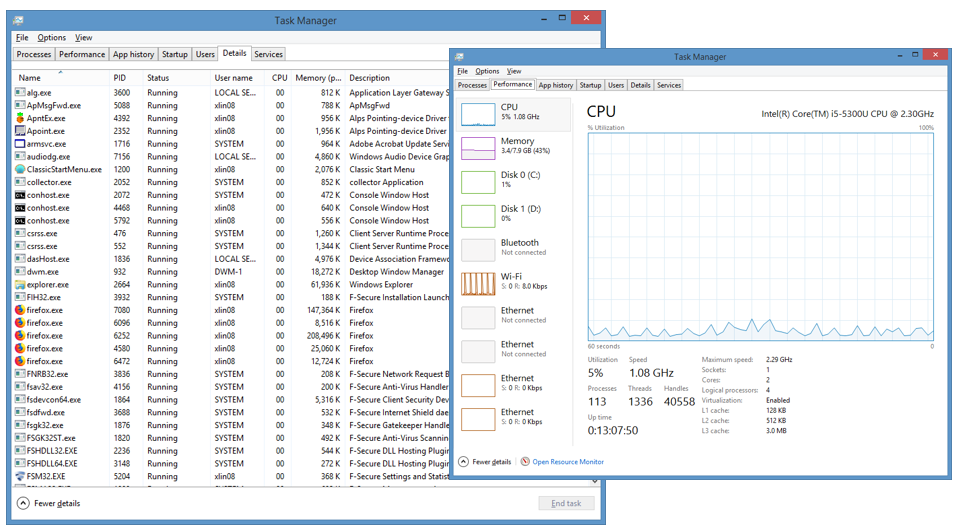
\includegraphics[scale=0.6]{img/C2/2-1/1.png}
	\caption{Windows进程}
\end{figure}

进程指的是一个具有一定独立功能的程序关于某个数据集合的一次运行活动。进程是系统进行资源分配和调度运行的基本单位。进程实体中包含三个组成部分:

\begin{enumerate}
	\item 程序
	\item 数据
	\item 进程控制块(PCB, Process Control Block)
\end{enumerate}

程序(program)与进程是有区别的,程序是静态的,进程是动态的。当程序的可执行文件被装入内存后就会变成进程。进程可以认为是执行中的程序,进程需要一定资源(如CPU时间、内存、文件、I/O设备)完成任务。这些资源可以在创建的时候或者运行中分配。一个程序可以通过GUI(Graphic User Interface)图形用户界面的鼠标点击、CLI(Command-line Interface)命令行界面输入程序名等方式运行。

\begin{figure}[H]
	\centering
	
\includegraphics[]{img/C2/2-1/2.png}
	\caption{GUI图形用户界面}
\end{figure}

\begin{figure}[H]
	\centering
	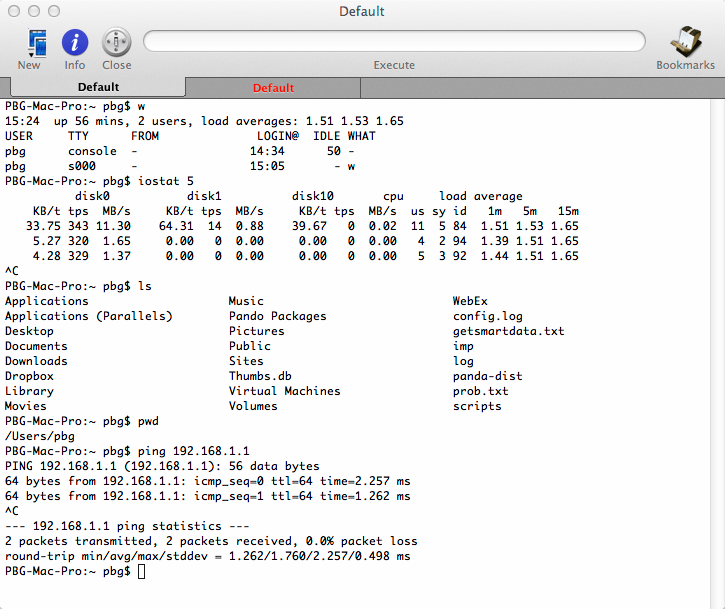
\includegraphics[scale=0.5]{img/C2/2-1/3.png}
	\caption{CLI命令行界面}
\end{figure}

\subsection{内存管理}

内存通常包括了栈区(stack)、堆区(heap)、数据区、程序代码区:

\begin{itemize}
	\item 栈区:由编译器自动分配和释放,存放函数的参数值、局部变量的值等。

	\item 堆区:一般由程序员分配和释放,若程序员不释放,程序结束后被OS回收。

	\item 数据区:存放全局变量和静态变量,程序结束后由系统释放。

	\item 程序代码区:存放函数体的二进制代码。
\end{itemize}

\begin{figure}[H]
	\centering
	\begin{tikzpicture}[scale=0.7]
		\draw[-] (0,0) -- (0,10) -- (5,10) -- (5,0) -- (0,0);
		\draw[-] (0,2) -- (5,2);
		\draw[-] (0,4) -- (5,4);
		\draw[-] (0,6) -- (5,6);
		\draw[-] (0,8) -- (5,8);

		\draw (0,0) node[left] {0};
		\draw (0,10) node[left] {max};

		\draw (2.5,1) node {Text};
		\draw (2.5,3) node {Data};
		\draw (2.5,5) node {Heap};
		\draw (2.5,9) node {Stack};

		\draw[->] (2.5,8) -- (2.5,7.5);
		\draw[->] (2.5,6) -- (2.5,6.5);
	\end{tikzpicture}
	\caption{内存管理}
\end{figure}

\subsection{进程状态模型}

在两状态进程模型中,进程被分为运行态(running)和非运行态(not-running)。

\begin{figure}[H]
	\centering
	\begin{tikzpicture}[node distance=3cm,thick,auto]
		\node[state,initial] (s1) {非运行态};
		\node[state,accepting right,accepting text = {end}] (s2) [right of=s1] {运行态};

		\path[->] (s1) edge[bend left] node[above] {分配} (s2);
		\path[->] (s2) edge[bend left] node[below] {暂停} (s1);
	\end{tikzpicture}
	\caption{两态模型}
\end{figure}

并非所有进程只要是非运行态就一定处于就绪状态,有的需要阻塞等待I/O完成。因此非运行态又可分为就绪态(ready)和阻塞态(block)。 \\

所有的进程从其创建到销毁都有各自的生命周期,进程要经过如下几个阶段:

\begin{figure}[H]
	\centering
	\begin{tikzpicture}[node distance=4.5cm,thick,auto]
		\node[state,initial] (s1) {创建};
		\node[state] (s2)[below of=s1] {就绪};
		\node[state] (s3)[right of=s2] {执行};
		\node[state] (s4)[above of=s3] {阻塞};
		\node[state,accepting below,accepting text = {end}] (s5)[right of=s3] {释放};

		\path[->] (s1) edge node[left] {许可} (s2);
		\path[->] (s2) edge[bend left] node[above] {CPU调度} (s3);
		\path[->] (s3) edge[bend left] node[below] {时间片执行完} (s2);
		\path[->] (s3) edge node[right] {产生阻塞事件} (s4);
		\path[->] (s4) edge node[left] {解除阻塞} (s2);
		\path[->] (s3) edge node {终止} (s5);
	\end{tikzpicture}
	\caption{五态模型}
\end{figure}

\begin{enumerate}
	\item 创建状态:系统已经为其分配了PCB(可以获取进程的而信息),但是所需要执行的进程的上下文环境(context)还未分配,所以这个时候的进程还无法被调度。

	\item 就绪状态:该进程已经分配到除CPU之外的全部资源,并等待CPU调度。

	\item 执行状态:进程已获得CPU资源,开始正常提供服务。

	\item 阻塞状态:所有的进程不可能一直抢占CPU,依据资源调度的算法,每一个进程运行一段时间之后,都需要交出当前的CPU资源,给其它进程执行。

	\item 终止状态:某一个进程达到了自然终止的状态,或者进行了强制性的停止,那么进程将进入到终止状态,进程将不再被执行。
\end{enumerate}

\subsection{多进程}

Python中在进行多进程开发的时候可以使用multiprocessing模块进行多进程的编写,这个模块内容提供有一个Process类,利用这个类可以进行多进程的定义。所有的Python程序执行都是通过主进程开始的,所有通过Process定义的进程都属于子进程。 \\

\mybox{创建多进程}
\begin{lstlisting}[language=Python]
import multiprocessing

def worker():
	"""
		进程处理函数
	"""
	print("【进程】id:%d,名称:%s" % (
		multiprocessing.current_process().pid,
		multiprocessing.current_process().name)
	)

def main():
	print("【主进程】id:%d,名称:%s" % (
		multiprocessing.current_process().pid,
		multiprocessing.current_process().name)
	)

	# 创建3个进程
	for i in range(3):
		process = multiprocessing.Process(
			target=worker, name="进程%d" % i
		)
		process.start()

if __name__ == "__main__":
	main()
\end{lstlisting}

\begin{tcolorbox}
	\mybox{运行结果} \\
	【主进程】id:4476,名称:MainProcess \\
	【进程】id:14216,名称:进程0 \\
	【进程】id:1424,名称:进程1 \\
	【进程】id:16636,名称:进程2
\end{tcolorbox}

psutil是一个进程管理的第三方模块,该模块可以跨平台(Linux、UNIX、MaxOS、Windows都支持)地进行进程管理,可以极大地简化不同系统中的进程处理操作。 \\

\mybox{获取全部进程信息}
\begin{lstlisting}[language=Python]
import psutil

def main():
	# 获取全部进程
	for process in psutil.process_iter():
		print("【进程】id:%d,名称:%s,创建时间:%s" % (
			process.pid, process.name,
			process.create_time())
		)

if __name__ == "__main__":
	main()
\end{lstlisting}

\newpage

\section{进程控制块PCB}

\subsection{PCB(Process Control Block)}

进程控制块PCB是OS控制和管理进程时所用的基本数据结构,PCB是相关进程存在于系统中的唯一标志,系统根据PCB而感知相关进程的存在。 \\

PCB中包含了关于进程的一些信息,如进程标识(pid)、程序计数器、状态信息、CPU调度信息、内存管理信息、I/O状态信息等。 \\

Linux中C语言<linux/sched.h>头文件中定义的进程结构如下: \\

\mybox{进程结构}
\begin{lstlisting}[language=C]
pid t_pid;					/* process identifier */
long state;					/* state of the process */
unsigned int time_slice;	/* scheduling information */
struct task_struct *parent;	/* this process's parent */
struct list_head children;	/* this process's children */
struct files_struct *files;	/* list of open files */
struct mm_struct *mm;		/* address space */
\end{lstlisting}

\subsection{进程切换}

当CPU切换到另一个进程时,系统必须保存当前执行进程的上下文(context),并且加载需要被执行进程的上下文。进程的上下文都被保存在PCB中。

\begin{figure}[H]
	\centering
	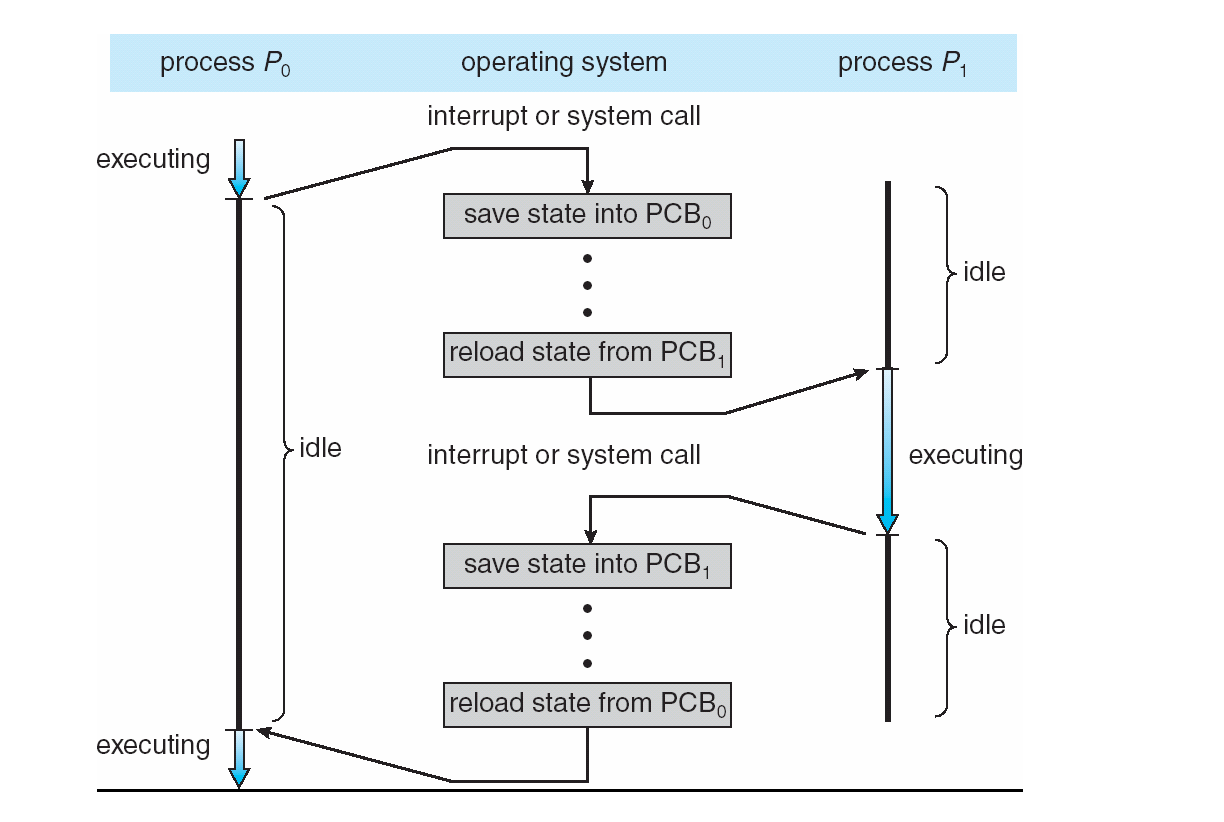
\includegraphics[scale=0.5]{img/C2/2-2/1.png}
	\caption{进程切换}
\end{figure}

\newpage

\section{线程}

\subsection{线程(Thread)}

60年代,在OS中能拥有资源和独立运行的基本单位是进程,然而随着计算机技术的发展,进程出现了很多弊端。由于进程是资源拥有者,创建、撤消与切换存在较大的时空开销。因此在80年代,出现了能独立运行的基本单位线程。 \\

线程是操作系统进行运算调度的最小单位,它被包含在进程中,是进程中的实际运作单位。一个进程中可以并发多个线程,每条线程并行执行不同的任务。

\begin{figure}[H]
	\centering
	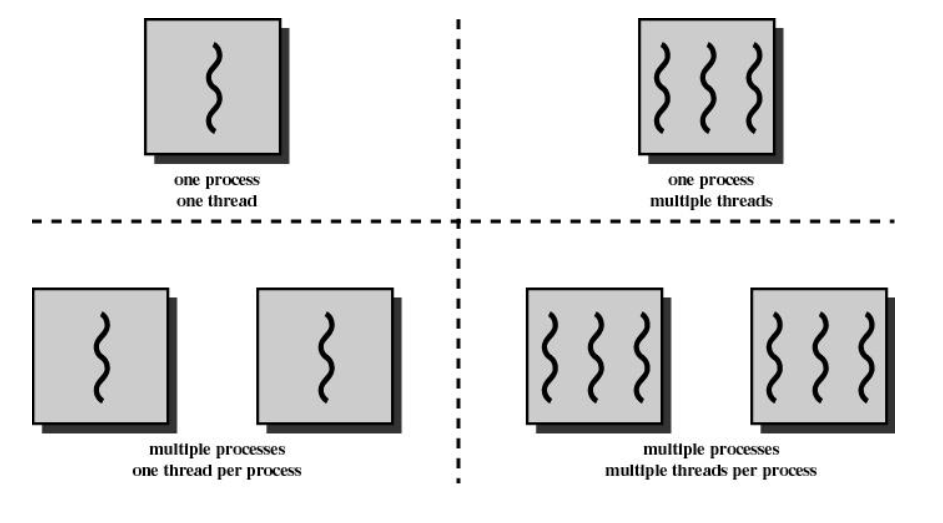
\includegraphics[scale=0.6]{img/C2/2-3/1.png}
	\caption{进程与线程的区别}
\end{figure}

由于线程比进程更小,基本上不拥有系统资源,故对它的调度所付出的开销就会小得多,能更高效的提高系统内多个程序间并发执行的程度,从而显著提高系统资源的利用率和吞吐量。因此使用线程可以带来很多好处:

\begin{itemize}
	\item 创建一个线程相比创建一个进程花费更少的时间。
	\item 结束一个线程相比结束一个进程花费更少的时间。
	\item 在同一个进程中切换不同线程花费更少的时间。
	\item 线程与资源分配无关,它属于某一个进程,与进程内其它线程一起共享进程资源。
\end{itemize}

\subsection{子进程(Child Process)}

fork()函数是UNIX或类UNIX中的分叉函数,fork()函数将运行着的程序分成两个几乎完全一样的进程,每个进程都启动一个从代码的同一位置开始执行的线程。这两个进程中的线程继续执行,就像是两个用户同时启动了该应用程序的两个副本。 \\

\mybox{创建子进程}
\begin{lstlisting}[language=C]
#include <stdio.h>
#include <sys/types.h>
#include <wait.h>
#include <unistd.h>

int main() {
	pid_t pid;

	pid = getpid();
	printf("Before fork(): pid is %d\n", pid);

	// fork a child process
	pid = fork();

	if(pid < 0) {               // error
		fprintf(stderr, "Fork failed.\n");
		return 1;
	} else if(pid == 0) {       // child process
		printf("Child process: pid is %d\n", getpid());
		execlp("/bin/ls", "ls", NULL);
	} else {                    // parent process
		printf("Parent process: pid is %d\n", getpid());
		wait(NULL);
		printf("Child completed.");
	}
	
	return 0;
}
\end{lstlisting}

\begin{tcolorbox}
	\mybox{运行结果} \\
	Before fork(): my pid is 2250 \\
	Parent Process: my pid is 2250 \\
	Child Process: my pid is 2251 \\
	main main.c \\
	Child Complete
\end{tcolorbox}

\begin{figure}[H]
	\centering
	\begin{tikzpicture}[node distance=3cm,thick,auto]
		\node[state,initial] (fork) {fork};
		\node[state] (execvp)[below of=fork] {execvp};
		\node[state] (ls)[below of=execvp] {ls};
		\node[state] (wait)[right of=fork] {wait};
		\node[state,accepting below,accepting text = {end}] (end)[right of=ls] {end};

		\path[->] (fork) edge node[left] {child} (execvp);
		\path[->] (execvp) edge node {} (ls);
		\path[->] (ls) edge node {} (end);
		\path[->] (fork) edge node {parent} (wait);
		\path[->] (wait) edge node {} (end);
	\end{tikzpicture}
	\caption{子进程}
\end{figure}

正常情况下,子进程由父进程创建,子进程可以再创建新的进程。父子进程是一个异步过程,父进程永远无法预测子进程的结束,所以,当子进程结束后,它的父进程会调用wait()或waitpid()取得子进程的终止状态,回收掉子进程的资源。 \\

但是一些情况下会产生僵尸进程(zoobie process)和孤儿进程(orphan process)的情况:

\begin{itemize}
	\item 僵尸进程:子进程退出了,但是父进程没有用wait()或waitpid()去获取子进程的状态信息,那么子进程的进程描述符仍然保存在系统中,这种进程称为僵尸进程。

	\item 孤儿进程:父进程结束了,而它的一个或多个子进程还在运行,那么这些子进程就成为了孤儿进程。子进程的资源由init进程(pid=1)回收。
\end{itemize}

\newpage

\section{进程调度}

\subsection{进程调度(Scheduling)}

\begin{enumerate}
	\item 短程调度(STS, Short Term Scheduling):从准备队列中选择进程送到CPU执行。

	\item 中程调度(MTS, Medium Term Scheduling):从将外存中挂起的进程中选择进程送到内存。

	\item 长程调度(LTS, Long Term Scheduling):从外存中选择一个作业送到内存中,为其创建进程,并加入准备队列。
\end{enumerate}

\begin{figure}[H]
	\centering
	\begin{tikzpicture}[node distance=5cm,thick,auto]
		\node[state,initial] (s1) {New};
		\node[state] (s2)[below of=s1] {Ready};
		\node[state] (s3)[right of=s2] {Running};
		\node[state] (s4)[below of=s3] {Waiting};
		\node[state] (s5)[left of=s4] {Suspended};
		\node[state,accepting below,accepting text = {end}] (s6)[right of=s3] {Terminated};

		\path[->] (s1) edge node[left] {admitted (LTS)} (s2);
		\path[->] (s2) edge[bend left] node[above] {scheduler dispatch (STS)} (s3);
		\path[->] (s3) edge[bend left] node[below] {interrupt} (s2);
		\path[->] (s3) edge node[right] {I/O or event waiting} (s4);
		\path[->] (s4) edge[bend left] node[below] {swapping out (MTS)} (s5);
		\path[->] (s5) edge node[left] {swapping in} (s2);
		\path[->] (s3) edge node {exit} (s6);
	\end{tikzpicture}
	\caption{进程调度}
\end{figure}

\subsection{调度准则(Scheduling Criteria)}

调度的基本准则分为面向用户和面向系统两方面。 \\

面向用户准则包括:

\begin{enumerate}
	\item 响应时间(response time)快:一般采用响应时间作为衡量调度算法的重要准则之一。从用户角度看,调度策略应尽量降低响应时间,使响应时间处在用户能接受的范围之内。

	\item 周转时间(turnaround time)短:周转时间是指从作业被提交给系统开始,到作业完成为止的这段时间间隔。通常把周转时间的长短作为评价批处理系统的性能、选择作业调度方式与算法的重要准则之一。

	\item 截止时间(deadline)的保证:截止时间是指某任务必须开始执行的最迟时间,或必须完成的最迟时间。截止时间是用于评价实时系统性能的重要指标。

	\item 优先权(priority)准则:让某些紧急的作业能得到及时处理,在要求较严格的场合,往往还须选择抢占式调度方式(preemptive),才能保证紧急作业得到及时处理。
\end{enumerate}

面向系统准则包括:

\begin{enumerate}
	\item 系统吞吐量(throughput)高:吞吐量是指在单位时间内系统所完成的作业数。

	\item 处理机利用率高:使处理机的利用率成为衡量系统性能的十分重要的指标。

	\item 各类资源的平衡利用:有效地利用其它各类资源,如内存、外存和 I/O 设备等。

	\item 公平性(fariness):不能让某一些进程遭受饥饿。
\end{enumerate}

\subsection{决策模式(Decision Mode)}

OS调度算法的决策模式分为非抢占式(nonpreemptive)和抢占式(preemptive)。

\begin{itemize}
	\item 非抢占式:一个进程一旦开始执行就会一直占用处理机,直到进程结束或发生阻塞。非抢占式主要用于批处理系统。

	\item 抢占式:当前正在运行的进程可以被打断,并转移到就绪态,可防止单一进程长时间独占CPU。抢占式主要用于实时性要求较高的实时系统以及性能要求较高的批处理系统和分时系统。
\end{itemize}

\subsection{先来先服务(FCFS, First Come First Serve)}

最简单的CPU调度算法是FCFS算法,FCFS策略可以通过FIFO队列容易地实现。当一个进程进入就绪队列时,它的PCB会被链接到队列尾部。当CPU空闲时,它会分配给位于队列头部的进程,并且将这个进程从队列中移去。 \\

FCFS策略的缺点是平均等待时间往往很长。 \\

假设有一组进程,它们在时间0到达:

\begin{table}[H]
	\centering
	\setlength{\tabcolsep}{5mm}{
		\begin{tabular}{|c|c|}
			\hline
			\textbf{进程} & \textbf{执行时间(ms)} \\
			\hline
			$ P_1 $       & 24                      \\
			\hline
			$ P_2 $       & 3                       \\
			\hline
			$ P_3 $       & 3                       \\
			\hline
		\end{tabular}
	}
\end{table}

如果进程按$ P_1 $、$ P_2 $、$ P_3 $的顺序到达,Gantt图如下:

\begin{figure}[H]
	\centering
	\begin{tikzpicture}[scale=0.5]
		\draw[-] (0,0) -- (30,0) -- (30,3) -- (0,3) -- (0,0);
		\draw[-] (24,0) -- (24,3);
		\draw[-] (27,0) -- (27,3);

		\draw (0,0) node[below] {0};
		\draw (24,0) node[below] {24};
		\draw (27,0) node[below] {27};
		\draw (30,0) node[below] {30};

		\draw (12,1.5) node {$ P_1 $};
		\draw (25.5,1.5) node {$ P_2 $};
		\draw (28.5,1.5) node {$ P_3 $};
	\end{tikzpicture}
\end{figure}

进程$ P_1 $的等待时间为0,进程$ P_2 $的等待时间为24,而进程$ P_3 $的等待时间为27。因此,平均等待时间为$ (0 + 24 + 27) / 3 = 17 $ ms。 \\

不过,如果进程按$ P_2 $、$ P_3 $、P1的顺序到达,Gantt图如下:

\begin{figure}[H]
	\centering
	\begin{tikzpicture}[scale=0.5]
		\draw[-] (0,0) -- (30,0) -- (30,3) -- (0,3) -- (0,0);
		\draw[-] (3,0) -- (3,3);
		\draw[-] (6,0) -- (6,3);

		\draw (0,0) node[below] {0};
		\draw (3,0) node[below] {3};
		\draw (6,0) node[below] {6};
		\draw (30,0) node[below] {30};

		\draw (1.5,1.5) node {$ P_2 $};
		\draw (4.5,1.5) node {$ P_3 $};
		\draw (18,1.5) node {$ P_1 $};
	\end{tikzpicture}
\end{figure}

现在平均等待时间为$ (0 + 3 + 6) / 3 = 3$ ms,这个减少是相当大的。 \\

FCFS算法特点如下:

\begin{itemize}
	\item 算法思想:主要从公平的角度考虑(类似生活中的排队)

	\item 算法规则:按照进程到达的先后顺序进行服务

	\item 决策模式:非抢占式

	\item 优点:公平、算法实现简单

	\item 缺点:排在长作业后面的短作业需要等待很长时间,带权周转时间很大,对短作业来说用户体验不好
\end{itemize}

\subsection{最短作业优先(SJF, Shortest Job First)}

SJF算法是最优的,因为进程的平均等待时间最小。通过将短进程移到长进程之前,短进程的等待时间减少大于长进程的等待时间增加。因而,平均等待时间减少。 \\

SJF算法的真正困难是如何知道下次CPU执行的长度。一种方法是预测下一个CPU执行的长度,可以认为下一个CPU执行的长度与以前的相似。因此,通过计算下一个CPU执行长度的近似值,可以选择具有预测最短CPU执行的进程来运行。 \\

SJF算法可以是抢占或非抢占的。当一个新进程到达就绪队列而以前进程正在执行时,就需要选择了。新进程的下次CPU执行,与当前运行进程的尚未完成的CPU执行相比,可能还要小。抢占SJF算法会抢占当前运行进程,而非抢占SJF算法会允许当前运行进程先完成CPU执行。抢占SJF调度有时称为最短剩余时间优先调度(Shortest Remaining Time First)。 \\

假设有一组进程:

\begin{table}[H]
	\centering
	\setlength{\tabcolsep}{5mm}{
		\begin{tabular}{|c|c|c|}
			\hline
			\textbf{进程} & \textbf{到达时间} & \textbf{执行时间(ms)} \\
			\hline
			$ P_1 $       & 0                 & 8                       \\
			\hline
			$ P_2 $       & 1                 & 4                       \\
			\hline
			$ P_3 $       & 2                 & 9                       \\
			\hline
			$ P_4 $       & 3                 & 5                       \\
			\hline
		\end{tabular}
	}
\end{table}

使用抢占SJF调度算法的Gantt图如下:

\begin{figure}[H]
	\centering
	\begin{tikzpicture}[scale=0.5]
		\draw[-] (0,0) -- (26,0) -- (26,3) -- (0,3) -- (0,0);
		\draw[-] (1+0.5,0) -- (1+0.5,3);
		\draw[-] (5,0) -- (5,3);
		\draw[-] (10,0) -- (10,3);
		\draw[-] (17,0) -- (17,3);

		\draw (0,0) node[below] {0};
		\draw (1+0.5,0) node[below] {1};
		\draw (5,0) node[below] {5};
		\draw (10,0) node[below] {10};
		\draw (17,0) node[below] {17};
		\draw (26,0) node[below] {26};

		\draw (0.5+0.25,1.5) node {$ P_1 $};
		\draw (3,1.5) node {$ P_2 $};
		\draw (7.5,1.5) node {$ P_4 $};
		\draw (13.5,1.5) node {$ P_1 $};
		\draw (21.5,1.5) node {$ P_3 $};
	\end{tikzpicture}
\end{figure}

进程$ P_1 $在时间0开始,因为这时只有进程$ P_1 $。进程$ P_2 $在时间1到达。进程$ P_1 $剩余时间(7 ms)大于进程$ P_2 $需要的时间(4 ms),因此进程$ P_1 $被抢占,而进程$ P_2 $被调度。 \\

抢占SJF调度的平均等待时间为$ [(10-1) + (1-1) + (17-2) + (5-3)] / 4 = 26 / 4 = 6.5$ ms。 \\

如果使用非抢占SJF调度,平均等待时间为$ 7.75 $ ms。

\subsection{优先级调度(Priority Scheduling)}

优先级调度算法的原理是给每个进程赋予一个优先级,每次需要进程切换时,找一个优先级最高的进程进行调度。这样,如果赋予长进程一个高优先级,则该进程就不会再饥饿(starvation)。 \\

优先级调度的优点是可以赋予重要的进程高优先级以确保重要任务能够得到CPU时间。其缺点是低优先级的进程可能会饥饿。不过,只要动态地调节优先级即可。例如,在一个进程执行特定CPU时间后将其优先级降低一个级别,或者将处于等待进程的优先级提高一个级别。这样,一个进程如果等待时间很长,其优先级将因持续提升而超越其他进程的优先级,从而得到CPU时间。 \\

假设有一组进程:

\begin{table}[H]
	\centering
	\setlength{\tabcolsep}{5mm}{
		\begin{tabular}{|c|c|c|}
			\hline
			\textbf{进程} & \textbf{执行时间(ms)} & \textbf{优先级} \\
			\hline
			$ P_1 $       & 10                      & 3               \\
			\hline
			$ P_2 $       & 1                       & 1               \\
			\hline
			$ P_3 $       & 2                       & 4               \\
			\hline
			$ P_4 $       & 1                       & 5               \\
			\hline
			$ P_5 $       & 5                       & 2               \\
			\hline
		\end{tabular}
	}
\end{table}

使用抢占优先级调度算法的Gantt图如下:

\begin{figure}[H]
	\centering
	\begin{tikzpicture}[scale=0.5]
		\draw[-] (0,0) -- (19,0) -- (19,3) -- (0,3) -- (0,0);
		\draw[-] (1+0.5,0) -- (1+0.5,3);
		\draw[-] (6,0) -- (6,3);
		\draw[-] (16-1,0) -- (16-1,3);
		\draw[-] (18-1,0) -- (18-1,3);

		\draw (0,0) node[below] {0};
		\draw (1+0.5,0) node[below] {1};
		\draw (6,0) node[below] {6};
		\draw (16-1,0) node[below] {16};
		\draw (18-1,0) node[below] {18};
		\draw (19,0) node[below] {19};

		\draw (0.5+0.25,1.5) node {$ P_2 $};
		\draw (3.5,1.5) node {$ P_5 $};
		\draw (11-0.5,1.5) node {$ P_1 $};
		\draw (17-1,1.5) node {$ P_3 $};
		\draw (18.5-0.5,1.5) node {$ P_4 $};
	\end{tikzpicture}
\end{figure}

平均等待时间为$ (6 + 0 + 16 + 18 + 1) / 5 = 8.2 $ ms。

\subsection{轮转调度(RR, Round Robin)}

RR调度算法是专门为分时系统设计的,它类似于FCFS调度,但是增加了抢占以切换进程。RR算法中,将一个较小时间单元定义为时间量(time quantum)或时间片(time slice),时间片的大小通常为$ 10 \sim 100 $ ms。 \\

就绪队列作为循环队列,CPU调度程序循环整个就绪队列,为每个进程分配不超过一个时间片的CPU。 \\

有两种情况可能发生:

\begin{enumerate}
	\item 进程可能只需少于时间片的CPU执行:进程本身会自动释放CPU,调度程序接着处理就绪队列的下一个进程。

	\item 当前运行进程的CPU执行大于一个时间片:时间片用完,进行上下文切换,再将进程加到就绪队列的尾部,接着CPU调度程序会选择就绪队列内的下一个进程。
\end{enumerate}

不过采用RR策略的平均等待时间通常较长。 \\

假设有一组进程,它们在时间0到达:

\begin{table}[H]
	\centering
	\setlength{\tabcolsep}{5mm}{
		\begin{tabular}{|c|c|}
			\hline
			\textbf{进程} & \textbf{执行时间(ms)} \\
			\hline
			$ P_1 $       & 24                      \\
			\hline
			$ P_2 $       & 3                       \\
			\hline
			$ P_3 $       & 3                       \\
			\hline
		\end{tabular}
	}
\end{table}

如果使用4 ms的时间片,那么$ P_1 $会执行最初的4 ms。由于它还需要20 ms,所以在第一个时间片之后它会被抢占,而CPU就交给队列中的下一个进程。由于$ P_2 $不需要4 ms,所以在其时间片用完之前就会退出。CPU接着交给下一个进程$ P_3 $。在每个进程都得到了一个时间片之后,CPU又交给了进程$ P_1 $以便继续执行。

\begin{figure}[H]
	\centering
	\begin{tikzpicture}[scale=0.5]
		\draw[-] (0,0) -- (30,0) -- (30,3) -- (0,3) -- (0,0);
		\draw[-] (4,0) -- (4,3);
		\draw[-] (7,0) -- (7,3);
		\draw[-] (10,0) -- (10,3);
		\draw[-] (14,0) -- (14,3);
		\draw[-] (18,0) -- (18,3);
		\draw[-] (22,0) -- (22,3);
		\draw[-] (26,0) -- (26,3);

		\draw (0,0) node[below] {0};
		\draw (4,0) node[below] {4};
		\draw (7,0) node[below] {7};
		\draw (10,0) node[below] {10};
		\draw (14,0) node[below] {14};
		\draw (18,0) node[below] {18};
		\draw (22,0) node[below] {22};
		\draw (26,0) node[below] {26};
		\draw (30,0) node[below] {30};

		\draw (2,1.5) node {$ P_1 $};
		\draw (5.5,1.5) node {$ P_2 $};
		\draw (8.5,1.5) node {$ P_3 $};
		\draw (12,1.5) node {$ P_1 $};
		\draw (16,1.5) node {$ P_1 $};
		\draw (20,1.5) node {$ P_1 $};
		\draw (24,1.5) node {$ P_1 $};
		\draw (28,1.5) node {$ P_1 $};
	\end{tikzpicture}
\end{figure}

平均等待时间为$ [(10-4) + 4 + 7] / 3 = 17 / 3 = 5.66 $ ms。 \\

RR算法的性能很大程度取决于时间片的大小。在一种极端情况下,如果时间片很大,那么RR算法与FCFS算法一样。相反,如果时间片很小,那么RR算法会导致大量的上下文切换。

\newpage

\section{进程间通信}

\subsection{进程管道通信}

进程是程序运行的基本单位,每一个程序内部都有属于自己的存储数据和程序单元,每一个进程都是完全独立的,彼此之前不能直接进行访问。但是可以通过一个特定的管道实现I/O。

\begin{figure}[H]
	\centering
	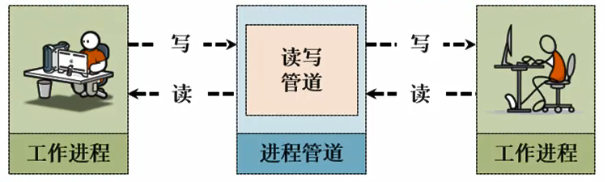
\includegraphics[]{img/C2/2-5/1.png}
	\caption{进程间通信}
\end{figure}

\mybox{创建进程通讯管道}
\begin{lstlisting}[language=Python]
import multiprocessing

def send_data(pipe, data):
	"""
		往管道发送数据
		Args:
			pipe (Pipe): 管道
			data (str): 发送的数据
	"""
	pipe.send(data)
	print("【进程%d】发送数据:%s" % (
		multiprocessing.current_process().pid,
		data
	))

def recv_data(pipe):
	"""
		从管道接收数据
		Args:
			pipe (Pipe): 管道
	"""
	print("【进程%d】接收数据:%s" % (
		multiprocessing.current_process().pid, 
		pipe.recv()
	))

def main():
	# 管道分为发送端和接收端
	send_end, recv_end = multiprocessing.Pipe()
	# 创建两个子进程,将管道传递到对应的处理函数
	sender = multiprocessing.Process(
				target=send_data,
				args=(send_end, "Hello!")
			)
	receiver = multiprocessing.Process(
				target=recv_data,
				args=(recv_end,)
			)
	sender.start()
	receiver.start()

if __name__ == "__main__":
	main()
\end{lstlisting}

\begin{tcolorbox}
	\mybox{运行结果} \\
	【进程11664】发送数据:Hello! \\
	【进程1032】接收数据:Hello!
\end{tcolorbox}

\subsection{生产者/消费者问题(Producer/Consumer Problem)}

不同的进程彼此之间可以利用管道实现数据的发送和接收,但是如果发送的数据过多并且接收处理缓慢的时候,这种情况下就需要引入队列的形式来进行缓冲的操作。

\begin{figure}[H]
	\centering
	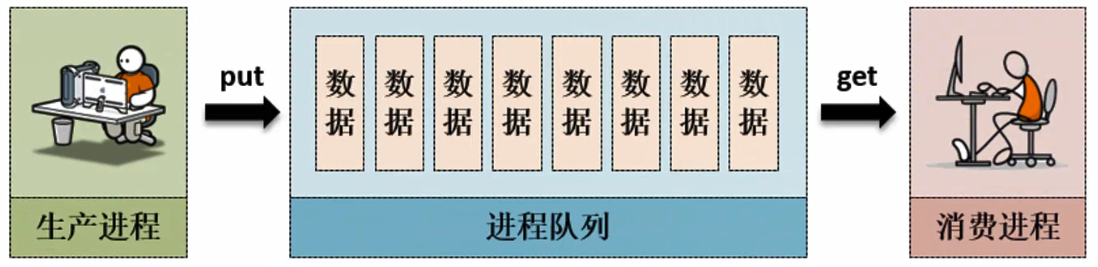
\includegraphics[scale=0.6]{img/C2/2-5/2.png}
	\caption{生产者/消费者问题}
\end{figure}

multiprocessing.Queue是Python多进程编程中提供的进程队列结构,该队列采用FIFO的形式实现不同进程间的数据通讯,这样可以保证多个数据可以按序实现发送与接收处理。 \\

\mybox{进程队列}
\begin{lstlisting}[language=Python]
import multiprocessing
import time

def produce(queue):
	"""
		生产数据
		Args:
			queue (Queue): 进程队列
	"""
	# 生产3条数据
	for item in range(3):
		time.sleep(2)
		data = "data-%d" % item
		print("【%s】生产数据:%s" % (
			multiprocessing.current_process().name,
			data
		))
		queue.put(data)

def consume(queue):
	"""
		消费数据
		Args:
			queue (Queue): 进程队列
	"""
	while True:     # 持续消费
		print("【%s】消费数据:%s" % (
			multiprocessing.current_process().name,
			queue.get()
		))

def main():
	queue = multiprocessing.Queue()
	producer = multiprocessing.Process(
				target=produce, name="Producer",
				args=(queue,)
			)
	consumer = multiprocessing.Process(
				target=consume, name="Consumer",
				args=(queue,)
			)
	producer.start()
	consumer.start()

if __name__ == "__main__":
	main()
\end{lstlisting}

\begin{tcolorbox}
	\mybox{运行结果} \\
	【Producer】生产数据:data-0 \\
	【Consumer】消费数据:data-0 \\
	【Producer】生产数据:data-1 \\
	【Consumer】消费数据:data-1 \\
	【Producer】生产数据:data-2 \\
	【Consumer】消费数据:data-2
\end{tcolorbox}

\newpage

\section{互斥与同步}

\subsection{互斥与同步}

计算机运行过程中,大量的进程在使用有限、独占、不可抢占的资源,由于进程无限,资源有限,这种矛盾称为竞争(race)。 \\

竞争条件分为两类:

\begin{enumerate}
	\item 互斥(mutex):两个或多个进程彼此之间没有内在的制约关系,但是由于要抢占使用某个临界资源(不能被多个进程同时使用的资源,如打印机)而产生制约关系。

	\item 同步(synchronization):两个或多个进程彼此之间存在内在的制约关系(前一个进程执行完,其他的进程才能执行)。
\end{enumerate}

在整个操作系统之中每一个进程都有自己独立的数据存储单元,也就是说不同进程之间无法直接实现数据共享。通过管道流可以实现进程之间的数据共享,相当于打通了不同进程之间的限制。但是不同的进程操作同一个资源就必须考虑数据同步的问题。 \\

要理解同步概念,首先要清楚进程不同步所带来的问题。 \\

\mybox{售票操作(Bug版本)}
\begin{lstlisting}[language=Python]
import multiprocessing
import time

def sell_ticket(dict):
	while True:     # 持续售票
		# 获取当前剩余票数
		num = dict.get("ticket")
		
		if num > 0:         # 如果还有票剩余
			time.sleep(1)   # 模拟网络延迟
			num -= 1        # 票数减1
			print("【售票员%d】售票成功,剩余票数:%d" % (
				multiprocessing.current_process().pid,
				num
			))
			dict.update({"ticket":num})     # 更新票数
		else:                				# 已经没有票了
			break

def main():
	# 创建共享数据对象
	manager = multiprocessing.Manager()
	# 创建一个可以被多个进程共享的字典对象
	ticket_dict = manager.dict(ticket=5)   # 默认有5张票

	# 创建多个售票进程
	sellers = [
		multiprocessing.Process(
			target=sell_ticket, args=(ticket_dict,)
		) 
		for _ in range(5)
	]

	for seller in sellers:
		seller.start()
	for seller in sellers:
		seller.join()   # 进程强制执行

if __name__ == "__main__":
	main()
\end{lstlisting}

\begin{tcolorbox}
	\mybox{运行结果} \\
	【售票员9732】售票成功,剩余票数:4 \\
	【售票员1640】售票成功,剩余票数:4 \\
	【售票员5976】售票成功,剩余票数:4 \\
	【售票员8048】售票成功,剩余票数:4 \\
	【售票员10516】售票成功,剩余票数:4 \\
	【售票员9732】售票成功,剩余票数:3 \\
	【售票员1640】售票成功,剩余票数:3 \\
	【售票员5976】售票成功,剩余票数:3 \\
	【售票员8048】售票成功,剩余票数:3 \\
	【售票员10516】售票成功,剩余票数:3 \\
	【售票员9732】售票成功,剩余票数:2  \\
	【售票员1640】售票成功,剩余票数:2  \\
	【售票员5976】售票成功,剩余票数:2  \\
	【售票员8048】售票成功,剩余票数:2  \\
	【售票员10516】售票成功,剩余票数:2 \\
	【售票员9732】售票成功,剩余票数:1 \\
	【售票员1640】售票成功,剩余票数:1 \\
	【售票员5976】售票成功,剩余票数:1 \\
	【售票员8048】售票成功,剩余票数:1 \\
	【售票员10516】售票成功,剩余票数:1 \\
	【售票员1640】售票成功,剩余票数:0 \\
	【售票员9732】售票成功,剩余票数:0 \\
	【售票员5976】售票成功,剩余票数:0 \\
	【售票员8048】售票成功,剩余票数:0 \\
	【售票员10516】售票成功,剩余票数:0
\end{tcolorbox}

多个进程同时进行票数判断的时候,在没有及时修改票数的情况下,就会出现数据不同步的问题。这套操作由于没有对同步的限制,所以就造成了不同步的问题。 \\

解决互斥方法有两种:

\begin{enumerate}
	\item 忙等待(busy waiting):等着但是不停地检查测试,直达能进行为止。

	\item 睡眠与唤醒(sleep and wakeup):引入Semaphore信号量,为进程睡眠而设置,唤醒由其它进程引发。
\end{enumerate}

\subsection{临界区(Critical Section)}

临界资源是各进程采取互斥的方式,一次仅允许一个进程使用的共享资源。属于临界资源的有打印机、变量、缓冲区等。 \\

每个进程中访问临界资源的那段代码称为临界区,每次只允许一个进程进入临界区,进入后,不允许其它进程进入。不论是硬件临界资源还是软件临界资源,多个进程必须互斥的对它进行访问。使用临界区时,一般不允许其运行时间过长,只要运行在临界区的线程还没有离开,其它所有进入此临界区的线程都会被挂起而进入等待状态,因此会在一定程度上影响程序的运行性能。 \\

\mybox{临界区}
\begin{lstlisting}[language=C]
do {
	// entry section
	critical section
	// exit section
	remainder section
} while(true);
\end{lstlisting}

\subsection{Peterson算法}

Peterson算法是由Gary L. Peterson于1981年提出的一个实现互斥锁的并发算法,可以控制两个进程访问一个共享的单用户资源而不发生访问冲突。 \\

Peterson算法要求两个进程共享两个数据项: \\

\mybox{Peterson算法}
\begin{lstlisting}[language=C]
int turn;		// 表示哪个进程可以进入临界区
bool flag[2];	// 表示哪个进程准备进入临界区
\end{lstlisting}

\subsection{互斥锁(Mutex)}

互斥锁是用一种简单的加锁方法来控制对共享资源的访问,互斥锁只有两种状态,即上锁(lock / acquire)和解锁(unlock / release)。 \\

互斥锁必须设定为一个原子操作(atomic operation),这意味着操作系统保证了如果一个进程锁定了一个互斥量,没有其它进程在同一时间可以成功锁定这个互斥量。 \\

\mybox{互斥锁}
\begin{lstlisting}[language=C]
acquire() {
	while(!available) {
		;			//busy wait
	}
	available = false;
}

release() {
	available = true;
}

do {
	acquire()
	//critical section
	release()
	//remainder section
} while(true);
\end{lstlisting}

并发进程的执行如果要进行同步处理,那么就必须对一些核心代码进行同步。Python中提供了一个Lock同步锁机制,利用这种锁机制可以实现部分代码的同步锁定,保证每一次只允许有一个进程执行这部分的代码。

\begin{figure}[H]
	\centering
	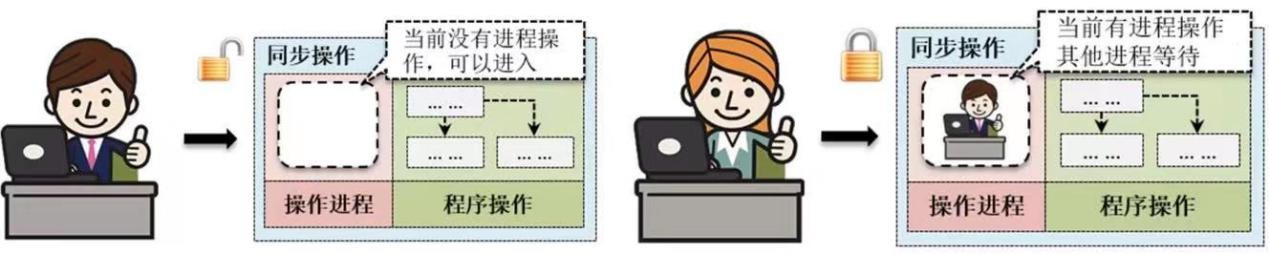
\includegraphics[]{img/C2/2-6/1.png}
	\caption{互斥锁}
\end{figure}

\mybox{售票操作(正确版本)}
\begin{lstlisting}[language=Python]
import multiprocessing
import time

def sell_ticket(lock, dict):
	while True:     # 持续售票
		# 请求锁定,如果5秒没有锁定则放弃
		lock.acquire(timeout=5)
		
		# 获取当前剩余票数
		num = dict.get("ticket")
		
		if num > 0:         # 如果还有票剩余
			time.sleep(1)   # 模拟网络延迟
			num -= 1        # 票数减1
			print("【售票员%d】售票成功,剩余票数:%d" % (
				multiprocessing.current_process().pid,
				num
			))
			dict.update({"ticket":num})     # 更新票数
		else:                # 已经没有票了
			break
		
		lock.release()      # 释放锁

def main():
	lock = multiprocessing.Lock()   # 同步锁
	# 创建共享数据对象
	manager = multiprocessing.Manager()
	# 创建一个可以被多个进程共享的字典对象
	ticket_dict = manager.dict(ticket=5)   # 默认有5张票

	# 创建多个售票进程
	sellers = [
		multiprocessing.Process(
			target=sell_ticket, args=(lock, ticket_dict)
		) 
		for _ in range(5)
	]

	for seller in sellers:
		seller.start()
	for seller in sellers:
		seller.join()   # 进程强制执行

if __name__ == "__main__":
	main()
\end{lstlisting}

\begin{tcolorbox}
	\mybox{运行结果} \\
	【售票员14612】售票成功,剩余票数:4 \\
	【售票员15868】售票成功,剩余票数:3 \\
	【售票员13972】售票成功,剩余票数:2 \\
	【售票员10844】售票成功,剩余票数:1 \\
	【售票员2872】售票成功,剩余票数:0
\end{tcolorbox}

一旦程序中追加了同步锁,那么程序的部分代码就只能以单进程执行了,这样势必会造成程序的执行性能下降,只有在考虑数据操作安全的情况下才会使用锁机制。

\subsection{硬件实现}

test\_and\_set()函数是用硬件保持的原子操作,这操作不会被打断。

\begin{lstlisting}[language=C]
bool test_and_set (bool *target) {
	bool rv = *target;
	*target = true;
	return rv;
}
\end{lstlisting}

共享锁lock初始化为false。while(test\_and\_set(\&lock));这句后面是的分号表示会循环等待解锁。

\begin{lstlisting}[language=C]
do {
	while(test_and_set(&lock)) {
		;		// do nothing
	}
	// critical section
	lock = false;
	// remainder section
} while(true);
\end{lstlisting}

compare\_and\_swap()函数也是按原子操作执行,不接受中断。

\begin{lstlisting}[language=C]
int compare_and_swap(int *value, int expected, int new_value) {
	int temp = *value;
	if(*value == expected) {
		*value = new_value;
	}
	returntemp;
}
\end{lstlisting}

互斥锁lock初始化为0。

\begin{lstlisting}[language=C]
do {
	while(compare_and_swap(&lock, 0, 1) != 0) {
		;		// do nothing
	}
	// critical section
	lock = 0;
	// remainder section
} while(true);
\end{lstlisting}

使用机器指令的优点是简单且易于证明,可以支持多个临界区,每个临界区都可以用它自己的变量定义。缺点是需要忙等待,并且可能会引发饥饿,当一个进程离开一个临界区并且有多个进程正在等待时,选择哪一个进程是任意的,因此可能会有进程被无限地拒绝进入。

\newpage

\section{Semaphore}

\subsection{Semaphore}

Semaphore(信号量)是一种有限资源的进程同步管理机制。例如银行的业务办理,所有客户都会拿到一个号码,而后号码会被业务窗口叫号,被叫号的办理者就可以办理业务。 \\

Semaphore类本质上是一种带有计数功能的进程同步机制,acquire()减少计数,release()增加计数。当可用信号量的计数为0时,后续进程将被阻塞。

\begin{figure}[H]
	\centering
	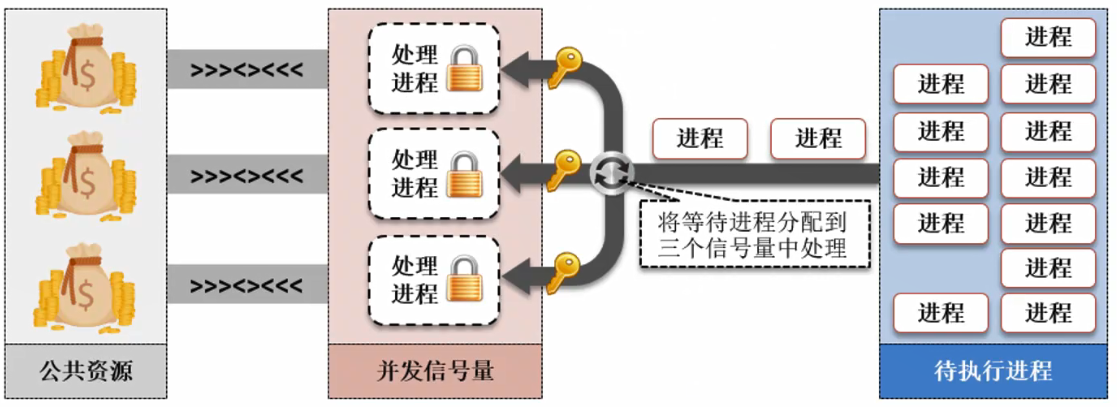
\includegraphics[scale=0.6]{img/C2/2-7/1.png}
	\caption{互斥锁}
\end{figure}

Lock一般是针对于一个资源同步的,而Semaphore是针对有限资源的并行访问。 \\

\mybox{信号量同步处理}
\begin{lstlisting}[language=Python]
import multiprocessing
import time

def work(sema):
	if sema.acquire():      # 获取信号量
		print("【进程%d】开始办理业务" % 
			multiprocessing.current_process().pid)
		time.sleep(2)       # 模拟办理业务
		print("【进程%d】结束办理业务" % 
			multiprocessing.current_process().pid)
		sema.release()      # 释放资源

def main():
	# 允许3个进程并发执行
	sema = multiprocessing.Semaphore(3)
	workers = [
		multiprocessing.Process(target=work, args=(sema,))
		for _ in range(10)
	]

	for worker in workers:
		worker.start()
	for worker in workers:
		worker.join()

if __name__ == "__main__":
	main()
\end{lstlisting}

\begin{tcolorbox}
	\mybox{运行结果} \\
	【进程7880】开始办理业务 \\
	【进程3032】开始办理业务 \\
	【进程5412】开始办理业务 \\
	【进程7880】结束办理业务 \\
	【进程2876】开始办理业务 \\
	【进程3032】结束办理业务 \\
	【进程14076】开始办理业务 \\
	【进程5412】结束办理业务 \\
	【进程8816】开始办理业务 \\
	【进程2876】结束办理业务 \\
	【进程14076】结束办理业务 \\
	【进程7900】开始办理业务 \\
	【进程7860】开始办理业务 \\
	【进程8816】结束办理业务 \\
	【进程16252】开始办理业务 \\
	【进程7860】结束办理业务 \\
	【进程7900】结束办理业务 \\
	【进程972】开始办理业务 \\
	【进程16252】结束办理业务 \\
	【进程972】结束办理业务
\end{tcolorbox}

一个信号量Semaphore是一个整型量,除对其初始化外,它只能由两个原子操作wait()和signal()进行访问。wait()和signal()即早前使用的P/V操作,P/V的名称来源于荷兰文proberen(测试)和verhogen(增量)。

\begin{lstlisting}[language=C]
wait(s) {
	while(s <= 0) {
		;		// busy waiting
	}
	s--;
}

signal(s) {
	s++;
}
\end{lstlisting}

但这并不是信号量的最终实现,最终的信号量实现最好是能解决两个问题:

\begin{enumerate}
	\item 不能忙等
	\item 记录处于等待状态的进程数量
\end{enumerate}

为了避免进程忙等,wait()和signal()的定义需要进行修改。当一个进程执行wait()但发现信号量$ s <= 0 $时,它必须等待,这里的等待不是忙等,而是阻塞自己。当一个进程阻塞且等待信号量时,在其它进程执行signal()之后被重新执行。 \\

信号量的意义为:

\begin{itemize}
	\item $ s > 0 $:表示有s个资源可用。
	\item $ s = 0 $:表示无资源可用。
	\item $ s < 0 $:表示等待队列中有$ |s| $个进程。
\end{itemize}

为了定义基于阻塞(block)和唤醒(wakeup)的信号量,可以将信号量定义为如下结构:

\begin{lstlisting}[language=C]
typedef struct {
	int value;
	struct process *list;
} Semaphore;
\end{lstlisting}

无需忙等的wait() / signal():

\begin{lstlisting}[language=C]
wait(Semaphore *s) {
	s->value--;
	if(s->value < 0) {
		add this process to s->list;
		block();
	}
}

signal(Semaphore *s) {
	s->value++;
	if(s->value <= 0) {
		remove a process p from s->list;
		wakeup(p);
	}
}
\end{lstlisting}

\newpage

\section{死锁}

\subsection{死锁(Deadlock)}

计算机系统中有很多独占性的资源,在同一时刻只能每个资源只能由一个进程使用。死锁是指两个或两个以上的进程在执行过程中,由于竞争资源或者由于彼此通信而造成的一种永久阻塞的现象。若无外力作用,它们都将无法推进下去,此时称系统处于死锁状态。

\begin{figure}[H]
	\centering
	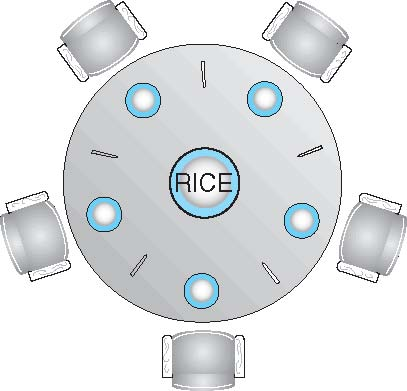
\includegraphics[]{img/C2/2-8/1.png}
	\caption{死锁}
\end{figure}

\subsection{哲学家就餐问题(Dining Philosophers Problem)}

假设有五位哲学家围坐在一张圆形餐桌旁,哲学家只做两件事情:吃饭或思考。餐桌上有一碗食物,每两个哲学家之间有一根筷子,哲学家必须用两根筷子才能吃东西。他们只能使用自己左右手边的那两根筷子。

\begin{figure}[H]
	\centering
	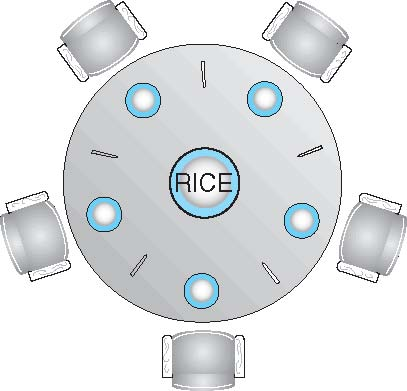
\includegraphics[]{img/C2/2-8/2.png}
	\caption{哲学家就餐问题}
\end{figure}

将5位哲学家分别编号为$ 0 ~ 4 $,第i位哲学家左手边的筷子编号为i。

\begin{lstlisting}[language=C]
do {
	wait(chopstick[i]);				// 申请左筷子
	wait(chopstick[(i + 1) % 5]);	// 申请右筷子
	// eat
	signal(chopstick[(i + 1) % 5]); // 释放右筷子
	signal(chopstick[i]);			// 释放左筷子
} while(true);
\end{lstlisting}

但是这个算法存在死锁的问题。每个哲学家都拿着左筷子,永远都在等右筷子(或者相反)。 \\

在实际的计算机问题中,缺乏筷子可以类比为缺乏共享资源。一种常用的计算机技术是资源加锁,用来保证在某个时刻,资源只能被一个程序或一段代码访问。当一个程序想要使用的资源已经被另一个程序锁定,它就等待资源解锁。当多个程序涉及到加锁的资源时,在某些情况下就有可能发生死锁。例如,某个程序需要访问两个文件,当两个这样的程序各锁了一个文件,那它们都在等待对方解锁另一个文件,而这永远不会发生。

\subsection{产生死锁的条件}

产生死锁必须要同时满足4个必要条件:

\begin{enumerate}
	\item 互斥(mutual exclusion):进程要求对所分配的资源进行排它性控制,即在一段时间内某资源仅有一个进程所占用。

	\item 占有并等待(hold and wait):当进程因请求资源而阻塞时,对已获得的资源保持不放。

	\item 不可剥夺(no preemption):进程已获得的资源在未使用完之前,不能剥夺,只能在使用完时由自己释放。

	\item 循环等待(circular wait):一定会有一个环互相等待。

	      \begin{figure}[H]
		      \centering
		      \begin{tikzpicture}[scale=4]
			      \node (p1)[process] at (0,2) {$ P_1 $};
			      \node (r1)[resource] at (1,2) {$ R_1 $};
			      \node (p2)[process] at (1,1) {$ P_2 $};
			      \node (r2)[resource] at (0,1) {$ R_2 $};

			      \draw[requested] (r1) -- (p1);
			      \draw[allocated] (r1) -- (p2);
			      \draw[requested] (r2) -- (p2);
			      \draw[allocated] (r2) -- (p1);
		      \end{tikzpicture}
		      \caption{循环等待}
	      \end{figure}
\end{enumerate}

\subsection{资源分配图(Resouce Allocation Graph)}

资源分配图是一种有向图,一个图$ G $可以由结点集$ V $以及边集$ E $组成。 \\

在资源分配图中,结点集$ V = P \cup R $,边集$ E = \{(P_i, R_i) \cup (R_i, P_i)\} $,其中$ P $为系统中所有进程的集合,$ R $为系统中所有资源类的集合。$ (P_i, R_i) $表示一条由进程$ P_i $到资源类$ R_i $的有向边,即进程$ P_i $申请资源$ R_i $,$ (R_i, P_i) $则是表示资源的分配。

\begin{figure}[H]
	\centering
	\begin{tikzpicture}[scale=4]
		\node (r1)[resource] at (1,2) {$ R_1 $};
		\node at (1,1.9) [circle,fill,inner sep=1.5pt]{};
		\node (r3)[resource] at (2,2) {$ R_3 $};
		\node at (2,1.9) [circle,fill,inner sep=1.5pt]{};

		\node (p1)[process] at (0.7,1.5) {$ P_1 $};
		\node (p2)[process] at (1.5,1.5) {$ P_2 $};
		\node (p3)[process] at (2.3,1.5) {$ P_3 $};

		\node (r2)[resource] at (1,1) {$ R_2 $};
		\node at (0.95,0.9) [circle,fill,inner sep=1.5pt]{};
		\node at (1.05,0.9) [circle,fill,inner sep=1.5pt]{};

		\draw[requested] (r1) -- (p1);
		\draw[allocated] (r1) -- (p2);
		\draw[requested] (r3) -- (p2);
		\draw[allocated] (r3) -- (p3);
		\draw[allocated] (r2) -- (p1);
		\draw[allocated] (r2) -- (p2);
	\end{tikzpicture}
	\caption{资源分配图}
\end{figure}

如果一个图中没有环路(回路),则系统中不存在死锁。若有环路,系统可能存在死锁。

\begin{figure}[H]
	\centering
	\begin{tikzpicture}[scale=4]
		\node (r1)[resource] at (1,2) {$ R_1 $};
		\node at (1,1.9) [circle,fill,inner sep=1.5pt]{};
		\node (r3)[resource] at (2,2) {$ R_3 $};
		\node at (2,1.9) [circle,fill,inner sep=1.5pt]{};

		\node (p1)[process] at (0.7,1.5) {$ P_1 $};
		\node (p2)[process] at (1.5,1.5) {$ P_2 $};
		\node (p3)[process] at (2.3,1.5) {$ P_3 $};

		\node (r2)[resource] at (1,1) {$ R_2 $};
		\node at (0.95,0.9) [circle,fill,inner sep=1.5pt]{};
		\node at (1.05,0.9) [circle,fill,inner sep=1.5pt]{};

		\draw[requested] (r1) -- (p1);
		\draw[allocated] (r1) -- (p2);
		\draw[requested] (r3) -- (p2);
		\draw[allocated] (r3) -- (p3);
		\draw[allocated] (r2) -- (p1);
		\draw[allocated] (r2) -- (p2);
		\draw[requested] (r2) -- (p3);
	\end{tikzpicture}
	\caption{死锁}
\end{figure}

\begin{figure}[H]
	\centering
	\begin{tikzpicture}[scale=4]
		\node (r1)[resource] at (1,2) {$ R_1 $};
		\node at (0.95,1.9) [circle,fill,inner sep=1.5pt]{};
		\node at (1.05,1.9) [circle,fill,inner sep=1.5pt]{};
		\node (r2)[resource] at (1,1) {$ R_2 $};
		\node at (0.95,0.9) [circle,fill,inner sep=1.5pt]{};
		\node at (1.05,0.9) [circle,fill,inner sep=1.5pt]{};

		\node (p1)[process] at (0,1.5) {$ P_1 $};
		\node (p2)[process] at (2,2) {$ P_2 $};
		\node (p3)[process] at (2,1.5) {$ P_3 $};
		\node (p4)[process] at (2,1) {$ P_4 $};

		\draw[requested] (r1) -- (p1);
		\draw[allocated] (r1) -- (p2);
		\draw[allocated] (r1) -- (p3);
		\draw[requested] (r2) -- (p3);
		\draw[allocated] (r2) -- (p1);
		\draw[allocated] (r2) -- (p4);
	\end{tikzpicture}
	\caption{有环路但非死锁}
\end{figure}

\newpage

\section{死锁的预防与避免}

\subsection{死锁预防}

可以通过破坏死锁产生的4个必要条件来预防死锁:

\begin{enumerate}
	\item 破坏``互斥"条件:由于资源互斥是资源使用的固有特性是无法改变的。

	\item 破坏``占有并等待"条件:每个进程在开始执行时就申请所需要的全部资源,只要有一个请求的资源不可用,其它可用资源就都不分配给它。采用该方法对系统来说是非常浪费的。

	\item 破坏``不可剥夺"条件:一个已拥有资源的进程,若它再提出新资源要求而不能立即得到满足时,它必须释放已经拥有的所有资源,以后需要时再重新申请。该方法实现复杂且要付出很大的代价,会导致之前的工作失效。

	\item 破坏``循环等待"条件:系统将所有资源按类型进行线性排序,并赋予不同的序号,所有进程对资源的请求必须严格按照资源序号递增的次序提出。该方法的缺点是进程实际需要资源的顺序不一定与资源的编号一致,因此仍会造成资源浪费。同时资源的序号必须相对稳定,从而限制了新设备的增加。
\end{enumerate}

\subsection{鸵鸟算法(Ostrich Algorithm)}

传说中鸵鸟看到危险就把头埋在地底下。当你对某一件事情没有一个很好的解决方法时,那就忽略它,装作看不到。这样的算法称为鸵鸟算法。 \\

鸵鸟算法可以称之为不是办法的办法。在计算机科学中,鸵鸟算法是解决潜在问题的一种方法。假设的前提是,这样的问题出现的概率很低。比如,在操作系统中,为应对死锁问题,可以采用这样的一种办法。大多数操作系统,包括UNIX、MINUX和Windows,处理死锁问题的办法仅仅是忽略它。其假设前提是大多数用户宁可在极偶然的情况下发生死锁也不愿接受性能的损失。因为解决死锁的问题,通常代价很大。所以鸵鸟算法,是平衡性能和复杂性而选择的一种方法。当死锁真正发生且影响系统正常运行时,采取手动干预——重新启动。

\begin{figure}[H]
	\centering
	
\includegraphics[scale=0.6]{img/C2/2-9/1.png}
	\caption{鸵鸟算法}
\end{figure}

\subsection{死锁避免}

死锁避免的基本思想就是在进行系统资源分配之前,先计算此次资源分配的安全性。若此次分配不会导致系统进入不安全状态,则将资源分配给进程,否则让进程等待。 \\

若系统能按某种顺序如$ <P_1, P_2, \dots, P_n> $来为每个进程分配其所需资源,直至最大需求,使每个进程都可顺序完成,则称系统处于安全状态(safe state)。若系统不存在这样一个安全序列,则称系统处于不安全状态(unsafe state)。 \\

只要系统处于安全状态,系统便不会进入死锁状态。当系统处于不安全状态时,并非所有不安全状态都必然转换为死锁。

\subsection{银行家算法(Banker's Algorithm)}

银行家算法可用于银行发放一笔贷款前,预测该笔贷款是否会引起银行资金周转问题。这里,银行的资源就类似于计算机系统的资源,贷款业务类似于计算机的资源分配。该算法可以预测一次资源分配对计算机系统是否是安全的。 \\

银行家算法需要设置以下数据结构:

\begin{enumerate}
	\item 可利用资源向量Available:一个具有$ m $个元素的数组,其中的每一个元素代表一类可利用资源的数目,其初始值为系统中该类资源的最大可用数目。其值将随着该类资源的分配与回收而动态改变。Available[j] = k表示系统中现有$ R_j $类资源$ k $个。

	\item 最大需求矩阵Max:一个$ n * m $的矩阵,定义了系统中$ n $个进程中每一个进程对$ m $类资源的最大需求。Max[i, j] = k表示进程$ i $对$ R_j $类资源的最大需求数目为$ k $个。

	\item 分配矩阵Allocation:一个$ n * m $的矩阵,定义了当前分配给每个进程的各类资源数量。Allocation[i, j] = k表示进程$ i $当前已分得$ R_j $类资源的数目为$ k $个。

	\item 需求矩阵Need:一个$ n * m $的矩阵,表示每一个进程尚需的各类资源数。Need[i, j] = k表示进程i还需要$ R_j $类资源$ k $个方能完成任务。
\end{enumerate}

矩阵间的关系为:

\vspace{-1cm}
\begin{align}\nonumber
	Need[i, j] = Max[i, j] - Allocation[i, j]
\end{align}

设$ Request_i $是进程$ P_i $的请求向量,$ Request_i[j] = k $表示进程$ P_i $需要$ k $个$ R_j $类资源。当进程$ P_i $发出资源请求后,系统按下述步骤进行检查:

\begin{enumerate}
	\item 如果$ Request_i \le Need_i $,则跳转到步骤2;否则,出错。

	\item 如果$ Request_i \le Available $,则跳转到步骤3;否则,表示尚无足够资源可供分配,进程$ P_i $必须阻塞等待。

	\item 系统试探性地将$ P_i $申请的资源分配给它,并修改下列数据:
	      \begin{align}\nonumber
		      Available  & = Available - Request[i]  \\ \nonumber
		      Allocation & = Allocation + Request[i] \\ \nonumber
		      Need[i]    & = Need[i] - Request[i]
	      \end{align}

	\item 系统利用安全性算法,检查此次资源分配以后,系统是否处于安全状态。若安全,才正式讲资源分配给进程$ P_i $。否则,试探分配失效,让进程$ P_i $阻塞等待。
\end{enumerate}

例如已知系统中进程的资源需求状况:

\begin{table}[H]
	\centering
	\setlength{\tabcolsep}{5mm}{
		\begin{tabular}{|c|c|c|}
			\hline
			\textbf{$ R_1 $} & \textbf{$ R_2 $} & \textbf{$ R_3 $} \\
			\hline
			9                & 3                & 6                \\
			\hline
		\end{tabular}
	}
	\caption{资源向量Resource}
\end{table}

\begin{table}[H]
	\centering
	\setlength{\tabcolsep}{5mm}{
		\begin{tabular}{|c|c|c|c|}
			\hline
			                 & \textbf{$ R_1 $} & \textbf{$ R_2 $} & \textbf{$ R_3 $} \\
			\hline
			\textbf{$ P_1 $} & 3                & 2                & 2                \\
			\hline
			\textbf{$ P_2 $} & 6                & 1                & 3                \\
			\hline
			\textbf{$ P_3 $} & 3                & 1                & 4                \\
			\hline
			\textbf{$ P_4 $} & 4                & 2                & 2                \\
			\hline
		\end{tabular}
	}
	\caption{最大需求矩阵Max}
\end{table}

\begin{table}[H]
	\centering
	\setlength{\tabcolsep}{5mm}{
		\begin{tabular}{|c|c|c|c|}
			\hline
			                 & \textbf{$ R_1 $} & \textbf{$ R_2 $} & \textbf{$ R_3 $} \\
			\hline
			\textbf{$ P_1 $} & 1                & 0                & 0                \\
			\hline
			\textbf{$ P_2 $} & 6                & 1                & 2                \\
			\hline
			\textbf{$ P_3 $} & 2                & 1                & 1                \\
			\hline
			\textbf{$ P_4 $} & 0                & 0                & 2                \\
			\hline
		\end{tabular}
	}
	\caption{分配矩阵Allocation}
\end{table}

根据最大需求矩阵Max与分配矩阵Allocation可计算得到需求矩阵Need:

\begin{table}[H]
	\centering
	\setlength{\tabcolsep}{5mm}{
		\begin{tabular}{|c|c|c|c|}
			\hline
			                 & \textbf{$ R_1 $} & \textbf{$ R_2 $} & \textbf{$ R_3 $} \\
			\hline
			\textbf{$ P_1 $} & 2                & 2                & 2                \\
			\hline
			\textbf{$ P_2 $} & 0                & 0                & 1                \\
			\hline
			\textbf{$ P_3 $} & 1                & 0                & 3                \\
			\hline
			\textbf{$ P_4 $} & 4                & 2                & 0                \\
			\hline
		\end{tabular}
	}
	\caption{需求矩阵Need}
\end{table}

根据资源向量Resource与分配矩阵Allocation可计算得到可用资源向量Available:

\begin{table}[H]
	\centering
	\setlength{\tabcolsep}{5mm}{
		\begin{tabular}{|c|c|c|}
			\hline
			\textbf{$ R_1 $} & \textbf{$ R_2 $} & \textbf{$ R_3 $} \\
			\hline
			0                & 1                & 1                \\
			\hline
		\end{tabular}
	}
	\caption{可用资源向量Available}
\end{table}

当前的可用资源为$ (0, 1, 1) $,如果将这些资源分配给$ P_1 $、$ P_3 $、$ P_4 $,并不能满足满足它们的需求。因为$ P_2 $只需要一份$ R_3 $资源就可以执行,执行结束后$ P_2 $会释放所有资源,那么可用资源变为$ (6, 2, 3) $。此时可用资源可以满足剩余任意一个进程,而都不会进入不安全状态。因此,$ <P_2, P_1, P_3, P_4> $就是其中的一个安全序列。 \\

如果无法找到一个安全序列,那么系统就处于不安全状态,便有可能进入死锁状态。

\newpage

\section{死锁的检测与解除}

\subsection{死锁检测与解除}

检测死锁不同于预防死锁,不限制资源访问方式和资源申请。OS可以周期性地执行死锁检测例程,检测系统中是否出现环路等待。 \\

当发现有进程死锁后,便应立即把它从死锁状态中解脱出来,常采用的方法有:

\begin{enumerate}
	\item 撤销进程法(abort):强制撤销部分、甚至全部死锁进程并剥夺这些进程的资源。撤销的原则可以按进程优先级和撤销进程代价的高低进行。

	\item 进程回退法(rollback):让一个或多个进程回退到足以回避死锁的地步,进程回退时自愿释放资源而不是被剥夺。要求系统保持进程的历史信息,设置还原点。
\end{enumerate}

\subsection{哲学家就餐问题(Dining Philosophers Problem)}

之前对于哲学家就餐问题的解决算法可能产生死锁。为了使全部哲学家都能进餐,算法必须避免死锁和饥饿。可行的解决方案是最多只允许4个哲学家同时进餐厅,则至少有1个哲学家可以拿到两根筷子进餐。进餐完毕后放下筷子,其他哲学家就可进餐,这样就不会出现死锁和饥饿。 \\

\mybox{哲学家就餐问题}
\begin{lstlisting}[language=C]
Semaphore capacity = 4;

Process phiosopher(i) {
	do {
	wait(capacity);						// 第5位哲学家将被阻塞
		wait(chopstick[i]);				// 申请左筷子
		wait(chopstick[(i +1) % 5]);	// 申请右筷子
		// eat
		signal(chopstick[(i + 1) % 5]);	// 释放右筷子
		signal(chopstick[i]);			// 释放左筷子
		signal(capacity);				// 唤醒被阻塞的哲学家
	} while(true);
}
\end{lstlisting}

\newpage